\section{Benchmark Design}
\label{sec:benchmark}

\fastkernels{} derives all tasks top-down from real model architectures, ensuring that every kernel can be traced to a specific layer in a specific model and evaluated end-to-end.

\subsection{Top-Down, Model-Driven Construction}
\label{sec:construction}

Unlike prior benchmarks that construct tasks bottom-up by combining primitive operators~\citep{kernelbench} or extracting subgraphs via automated pipelines~\citep{solexecbench}, \fastkernels{} takes a \emph{top-down} approach.
We begin with real model families---selected to represent the current and near-future frontier of AI workloads---and recursively decompose them into the kernels that constitute their inference paths.

\paragraph{Task construction.}
For each model architecture, we load the HuggingFace configuration and architecture definition, walk the forward pass, and produce standalone task implementations for each computational kernel with all configuration constants (hidden size, number of heads, data types) inlined from the model's configuration.
Every task is then audited to verify: (i)~semantic correctness of the reference implementation, (ii)~that the task captures the operator as it actually executes in the model (not a simplified proxy), (iii)~that tensor shapes and data types match the model's real configuration, and (iv)~that the task's interface matches the corresponding module in the production reference library (Section~\ref{sec:interface}).
The construction pipeline ships with \fastkernels{}, so users can add new architectures from HuggingFace with minimal effort.
No task is synthetic: unlike KernelBench's Level-2 random fusions or SOL-ExecBench's LLM-selected subgraphs, every task is an operation that runs in a real model during inference.

\subsection{Task Hierarchy}
\label{sec:hierarchy}

\fastkernels{} organizes tasks into four levels of increasing scope:

\begin{itemize}[leftmargin=*, itemsep=2pt, topsep=2pt]
\item \textbf{Level 1 --- Primitive operators.}
Individual operations: attention variants (GQA, MLA, sliding-window), normalizations (RMSNorm, LayerNorm), activations (SwiGLU, GeGLU), positional encodings (RoPE, ALiBi), and quantization/dequantization routines.

\item \textbf{Level 2 --- Fused operators.}
Multi-operation kernels representing natural fusion opportunities as they arise in real models: residual-add + RMSNorm + quantization, attention + output projection, MoE gate + dispatch + expert computation.

\item \textbf{Level 3 --- Full layers and blocks.}
Complete architectural blocks: transformer decoder layers, SSM scan blocks, MoE layers with routing, cross-attention layers, and vision encoder stages.

\item \textbf{Level 4 --- End-to-end model architectures.}
Full model inference paths evaluated as integrated systems.
The 47 representative architectures in Level~4 serve as the end-to-end evaluation set, but the underlying L1--L3 kernels cover most operators across ML models.
\end{itemize}

\paragraph{Standalone and composed evaluation.}
Crucially, the hierarchy is not just organizational---it is \emph{executable}.
L2--L4 baselines import their lower-level dependencies via relative imports (e.g., an L3 decoder layer does \texttt{from~..L2.attention~import~Attention}), mirroring how production frameworks assemble modules.
In \emph{standalone} mode (\texttt{-{}-standalone}), each candidate is benched in isolation: imported lower-level modules resolve to their production baselines regardless of what other candidate files exist.
In \emph{composed} mode, all candidate files in the candidate directory are active simultaneously, so an L3 block's lower-level imports resolve to agent-generated candidates rather than production baselines.
The standalone score measures how well the agent optimized one module; the composed score measures what a real deployment would observe when multiple agent-generated modules interact.
The gap between the two---the \emph{composition effect}---is a first-order signal that flat benchmarks are structurally unable to produce (Section~\ref{sec:eval-agents}).

\subsection{Architecture Coverage}
\label{sec:coverage}

\fastkernels{} is designed to cover as many model architectures as possible with the \emph{minimum} number of kernels, by consolidating near-identical operators (e.g., RoPE variants, normalizations, attention backends) into a single L1/L2 task and picking a small set of representative architectures whose union of operators subsumes the long tail of model families. The resulting 47 architectures span 8 categories and precision formats from 1.58-bit through FP32, and comprise 384 unique tasks: 108 L1, 155 L2, and 74 L3 kernel tasks, shared across architectures, plus the 47 end-to-end L4 models (Figure~\ref{fig:arch_pie}; counting rules and per-architecture details in Appendix~\ref{app:architectures}). 

To measure coverage, we implemented every architecture in HuggingFace Transformers (commit \texttt{89b6b17}) on \fastkernels{} without adding any operator: \textbf{94.6\% (472/499)} of them run and match native HF outputs within \texttt{dtype}-dependent tolerances, and only 5 require a genuinely new operation. The methodology and per-architecture results are in Appendix~\ref{app:hf_coverage}.



\begin{figure}[t]
\centering
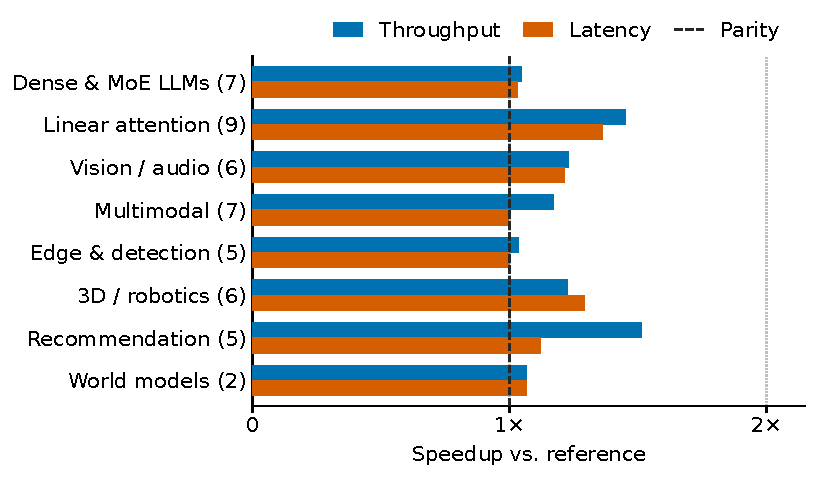
\includegraphics[width=0.7\linewidth]{figures/eval_e2e.pdf}
\caption{\textbf{Composition and reference performance of \fastkernels{}}: 47 end-to-end architectures across 8 categories (count in parentheses).
Each bar is the geometric-mean end-to-end speedup of \fastkernels{} over the production reference across the category's architectures (throughput and latency).
Per-architecture details in Appendix Tables~\ref{tab:arch_detail}, \ref{tab:bench_detail}, and~\ref{tab:bench_detail_b}.}
\label{fig:arch_pie}
\label{fig:eval-e2e}
\end{figure}

% Pie chart replaced by the category counts in Figure~\ref{fig:arch_pie} (space).
% \begin{figure}[t]
% \centering
% \begin{tikzpicture}[font=\footnotesize]
% \pie[radius=1.6, text=legend, color={
%   blue!55, orange!75, green!55, red!45, violet!55,
%   teal!60, cyan!50, brown!55, gray!55},
%   sum=auto, after number=]{
%   7/Dense \& MoE LLMs,
%   9/Linear Attention \& New Archs,
%   6/Vision / Video / Audio,
%   7/Multimodal \& Encoders,
%   5/Edge \& Detection,
%   6/3D / Robotics / Science,
%   5/Recommendation \& Specialized,
%   2/World Models}
% \end{tikzpicture}
% \caption{Composition of \fastkernels{}: 47 end-to-end architectures across 8 categories. Per-architecture details in Appendix Table~\ref{tab:arch_detail}.}
% \label{fig:arch_pie}
% \end{figure}

\subsection{Interface-Compatible Design}
\label{sec:interface}

A central design principle of \fastkernels{} is that optimized kernels should be deployable into existing production systems with minimal effort.
For each model architecture family, we identify the corresponding state-of-the-art production library (e.g., vLLM for LLMs, SGLang for serving) and design each task's interface---its \texttt{\_\_init\_\_} constructor signature and \texttt{forward} method---to closely match the corresponding module in that reference library.

A kernel optimized within \fastkernels{} can therefore be copied into vLLM, SGLang, or another production framework without interface refactoring.
Unlike FlashInfer-Bench's FIApply, which substitutes at the kernel dispatch level (an abstraction internal to FlashInfer), \fastkernels{}'s compatibility operates at the \emph{module} level, the unit production frameworks compose.

\subsection{Multi-GPU Communication Kernels}
\label{sec:multigpu}

Production inference at scale is almost always distributed, and its collectives and communication--computation overlaps materially affect end-to-end latency.
\fastkernels{} includes the communication path of its tensor-parallel models as tasks: the custom IPC all-reduce (L1); the tensor-parallel linear, embedding, and MoE layers that issue it (L2); and a decoder layer that fuses it with residual addition and RMSNorm (L3).
The all-reduce and row-parallel linear are benched in a real NCCL group of the capture's TP degree, and all of these operators run end to end inside models served at TP 2--8.
Dedicated benchmarks~\citep{commbench,parallelkernelbench} cover more communication patterns but score each program in isolation; \fastkernels{} places every collective in the schedule it shares with the model's compute kernels, where a kernel $1.5\times$ faster on one GPU can still slow the model.
